\documentclass[11pt, oneside]{article}   	% use "amsart" instead of "article" for AMSLaTeX format
\usepackage{geometry}                		% See geometry.pdf to learn the layout options. There are lots.
\geometry{letterpaper}                   		% ... or a4paper or a5paper or ... 
%\geometry{landscape}                		% Activate for for rotated page geometry
%\usepackage[parfill]{parskip}    		% Activate to begin paragraphs with an empty line rather than an indent
\usepackage{graphicx}				% Use pdf, png, jpg, or eps� with pdflatex; use eps in DVI mode
								% TeX will automatically convert eps --> pdf in pdflatex		
\usepackage{amssymb}
\usepackage{amsmath}
\usepackage{ifthen,version}
\newboolean{include-notes}
\usepackage[usenames,dvipsnames]{color}

% Comment out the following line to exclude the notes.
\setboolean{include-notes}{true}

\DeclareRobustCommand{\todo}[1]{\ifthenelse{\boolean{include-notes}}%
 {\textcolor{red}{\textbf{TODO: #1}}}{}}

\title{CHOMP Notes}
\author{Jennifer King}
%\date{}							% Activate to display a given date or no date

\begin{document}
\maketitle

\section*{CHOMP formalization}
Define a trajectory as a function which maps time to a configuration in configuration space:
\[ \xi : \left[0, 1\right] \rightarrow \mathcal{C} \subset \mathbb{R}^d \]
Then define an objective functional which maps trajectories to a real number:
\[ \mathcal{U} : \Xi \rightarrow \mathbb{R} \]
For CHOMP, the objective functional represents a tradeoff between two complementary aspects of motion planning.  The first penalizes a trajectory based on dynamic criteria such as velocity, acceleration or jerk.  The second penalizes a trajectory based on proximity to obstacles.  This is represented in the following equation:
\[ \mathcal{U}\left[\xi\right] = \mathcal{F}_{obs}\left[\xi\right] + \lambda\mathcal{F}_{smooth}\left[\xi\right] \]
where
\[ \mathcal{F}_{obs} : \Xi \rightarrow \mathbb{R} \]
\[ \mathcal{F}_{smooth} : \Xi \rightarrow \mathbb{R} \]
and $\lambda$ is a weighting factor which represents the tradeoff between the two sometimes conflicting functional values.  
\newline\newline
We can define the smoothness functional as the integration across the trajectory of any function which represents dynamic criteria.  One option, shown here, is to use squared velocity norms:
\begin{equation}\label{eq:f_smooth}
\mathcal{F}_{smooth} = \frac{1}{2} \int_0^1 \left\| \frac{d}{dt} \xi(t)\right\|^2 dt 
\end{equation}
\newline
Now define a function $x$ as follows:
\[x : \mathcal{C} \times \mathcal{B} \rightarrow \mathbb{R}^3 \]
which maps a configuration and body point to a point in the workspace.  If we then have a cost function:
\[ c : \mathbb{R}^3 \rightarrow \mathbb{R} \]
which assigns a cost to each point in the workspace, we can define the obstacle objective function:
\begin{equation}\label{eq:f_obs}
\mathcal{F}_{obs}\left[\xi\right] = \int_0^1 \int_{\mathcal{B}} c(x(\xi(t), u)) \left\| \frac{d}{dt} x(\xi(t), u) \right\| du dt 
\end{equation}
If we think about the arc length ($s$) between two points, $a$ and $b$, for a curve parameterized by $t$:
\[ s = \int_a^b \sqrt{\frac{dx}{dt}^2 + \frac{dy}{dt}^2} \]
Then its easy to see that the $\mathcal{F}_{obs}$ function multiplies the cost by the arc length rather than just doing a line integral.  This ensures that the obstacle objective is invariant to retiming the trajectory.  
\begin{figure}[here]
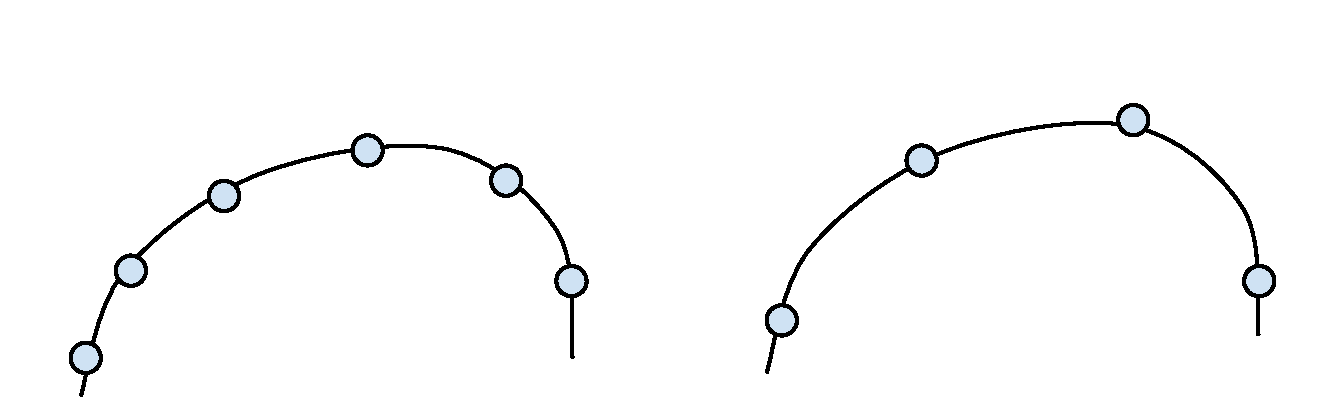
\includegraphics[width=\textwidth]{figs/invariant_objective}
\caption{The trajectories on the left and right have same length.  If cost was based on integrating across trajectory points, the left would have much higher cost.  Using arc length makes cost of each trajectory the same.}
\label{fig:invariant_objecive}
\end{figure}
Figure ~\ref{fig:invariant_objective} visualizes this point.
\newline
We want to use a traditional gradient descent algorithm to minimizes our object function $\mathcal{U}\left[\xi\right]$:
\[ \xi_{t+1} = \xi_t - \eta_i\bar{\nabla}\mathcal{F}\left[\xi\right] \]
To do this we must define the concept of functional gradient.  The functional gradient is the perturbation $\phi$ that causes maximal increase to the function.  Where:
\[ \phi : \left[0,1\right] \rightarrow \mathcal{C} \subset \mathbb{R}^d \]
In other words we want to find:
\[ \bar{\nabla}\mathcal{U} = \arg\max_{\phi}\;\mathcal{U}\left[\xi + \phi\right] \]
It can be seen from the above equation that the outcome of the maximization is heavily dependent on the size of $\phi$.  Because $\phi$ represents a normalized vector, this is equivalent to saying the outcome of the maximization is strongly dependent on our choose of norm.  \todo{Check this statement to be sure the understanding is correct.}
One option is the Euclidean norm.  For a vector $x \subset \mathbb{R}^n = \left(x_1,...,x_n\right)$:
\[\left\|x \right\| = \sqrt{\sum_{i=1}^n x_i^2} \]
For a trajectory:
\[\left\| \xi \right\| = \sqrt{\int_0^1 \xi(t) dt} \]
Using this as our norm, the Euclidean function gradient for a function $\mathcal{F}\left[\xi\right] = \int v(\xi(t))dt$ is:
\begin{equation}\label{eq:functional_gradient}
\bar{\nabla} \mathcal{F}\left[\xi\right] = \frac{\partial v}{\partial \xi} - \frac{d}{dt}\frac{\partial v}{\partial \xi'} 
\end{equation}
This is the Euler-Lagrange equation.
\newline
Now consider equation ~\ref{eq:f_smooth}.  Let:
\[v(\xi(t)) = \left\|\frac{d}{dt} \xi(t)\right\|^2 \]
Then \todo{Verify this}:
\[ \frac{\partial v}{\partial \xi} = 0 \]
\[ \frac{\partial v}{\partial \xi'} = 2\xi'(t) \]
\[ \frac{d}{dt} 2\xi'(t) = 2\frac{d^2}{dt^2} \xi(t) \]
By our definition:
\[\mathcal{F}_{smooth} = \frac{1}{2} \int v(\xi(t)) dt \]
So using equation ~\ref{eq:functional_gradient}:
\[ \bar{\nabla}\mathcal{F}_{smooth} = \frac{1}{2}\left(-2\frac{d^2}{dt^2}\xi(t)\right) = -\frac{d^2}{dt^2}\xi(t) \]
Next we consider equation ~\ref{eq:f_obs}. Let:
\[ v(\xi(t)) = \int_{\mathcal{B}} c(x(\xi(t), u)) \left\|\frac{d}{dt}x(\xi(t),u) \right\| du \]
\todo{Work out this math like we did the other}
\newline
Note: We formulated $\mathcal{F}_{smooth}$ and $\mathcal{F}_{obs}$ so that they did not rely on trajectory parameterization.  Thus none has been specified.  However, in order to do gradient descent, we had to pick a norm.  We picked Euclidean norm.  Because of this we have now created a dependency between our algorithm formulation and the choice of representation of the trajectory.  Specifically, we assume the trajectory function is represented in terms of a basis of Dirac delta functions so that the $i^{th}$ component is $\left<f, \delta_t\right> = \int f(\tau)\delta(t - \tau) d\tau = f(t)$. \todo{Explain this more}
\newline
\todo{Double check that these next two paragraphs accurately represent the content of section 3.3 of the journal paper}
\newline
The formulation above uses Euclidean norm specifically.  However this is not required.  What is required is that the norm we define over our space must depend solely on the dynamical quantities of the trajectory (in engish, only on the trajectory and its derivatives).  In other words, we want to define a norm as follows:
\[\left\|\xi\right\|^2_A = \int \sum_{n=1}^k \alpha_n(D^n\xi(t))^2 dt\]
Here $D^n$ is an $n^{th}$ order derivative operator and $\alpha_n \subset \mathbb{R}$ is a constant. If $k=1$ and $\alpha_1 = 1$ then:
\[\left\|\xi\right\|^2_A = \int \xi'(t)^2 dt \]
We can also define an inner product on two trajectories:
\[ \left<\xi_1, \xi_2\right> = \int \sum_{n=1}^k \alpha_n(D^n\xi_1(t))(D^n\xi_2(t)) dt \]
We use the $A$ operator only to differentiate this norm and dot product from the standard Euclidean norm.  $A$ must be constructed such that $A = D^TD$ where $D$ is a consituent differential operator \todo{What is this?} Then:
\[ \left<f, Af\right> = \int(Df(t))^2 dt \]

\section*{Identifying Parameterization}
In order to numerically perform a function gradient, a specific parameterization of the trajectory must be selected.  One choice is to sample from the trajectory at uniform time steps $\Delta t$: $\xi = \left[q_1^T,...,q_n^T\right]^T$.  We let $q_0$ represent the start configuration and $q_{n+1}$ represent the goal configuration.  Then the smoothness functional can be represented as:
\[ \mathcal{F}_{smooth} = \frac{1}{2(n+1)}\sum_{t=1}^{n+1} \left\| \frac{q_{t+1} - q_t}{\Delta t} \right\|^2 \]
We can generate an $n$ by $n$ differencing matrix $K$:
\[ K = \left[\begin{array}{ccccc}
1 & 0 & 0 & ... & 0 \\
0 & -1 & 1 & ... & 0 \\
. & . & . & . & . \\
0 & 0 & ... & -1 & 1 \\
0 & 0 & ... & 0 & -1 \\
\end{array}
\right]
\]
Then if we define a vector $e$ to handle endpoints conditions:
\[ e = \left[ \begin{array}{ccccc} -q_0 & 0 & ... & 0 & q_{n+1} \end{array} \right]^T \]
We can rewrite our smoothness function:
\[ \mathcal{F}_{smooth} = \frac{1}{2}\left\| K\xi + e \right\|^2 \]
Multiplying this out we get:
\[ \mathcal{F}_{smooth} = \frac{1}{2}( \xi^TK^TK\xi + 2\xi^TK^Te + e^Te) = \frac{1}{2}\xi^TA\xi + \xi^Tb + c \]
\end{document}  